% -------------------------------------------------------
% CTB FINAL REPORT
% 
% Author: Gabriel Villanova N. M.
% -------------------------------------------------------
\documentclass[letterpaper, 10pt, conference]{ieeeconf}

% IEEE config
\IEEEoverridecommandlockouts
\overrideIEEEmargins
\usepackage[hidelinks]{hyperref} 
\usepackage{listings}
\usepackage{caption}
\usepackage[newfloat]{minted}
\usepackage{graphicx}
\usepackage{float}
\usepackage{fullpage} 

\captionsetup[listing]{position=top}

% Title
\title{\LARGE \bf Capture The Bug 2023: RISC-V Verification Challenges}

% Author
\author{Gabriel Villanova Novaes Magalhães$^{1}$}

\begin{document}

% Title and Author
\maketitle
\thispagestyle{empty}
\pagestyle{empty}

% Sections
% -------------------------------------------------------
% Challenge Level 1 - Logical
% -------------------------------------------------------
\section{Challenge 1 Level 1 (C1L1): Logical}

For this challenge, two bugs were encountered, referred to as \textbf{1) Undefined Register} and \textbf{2) Incorrect Operand}. Both issues are presented below:

% ---------------------------
% BUG1
% ---------------------------
\subsection{Bug 1: Undefined Register}

\subsubsection{Cause}

The instruction, which is shown in Listing \ref{lst:invalid_reg} on line 15852 in ``test.S," contains a bug. RISC-V provides a standard set of 
register names, such as \texttt{x0}, \texttt{x1}, ..., \texttt{x31}, which are 32 general-purpose registers. These 
registers are named: zero, ra, sp, gp, tp, t0, t1, ..., s0, s1, ..., a0, a1, etc., and are valid registers. Since \texttt{z4} does not exist, the compiler returns an error.

\begin{listing}[h]
\caption{Invalid register instruction.}
\label{lst:invalid_reg}
\begin{minted}[frame=single]{nasm}
and s7, ra, z4 # line 15852 in test.S
\end{minted}
\end{listing}

\subsubsection{Solution}

In the test context, any of the valid registers can be used. Randomly, \texttt{z4} was replaced with the valid register \texttt{s4}, as presented in Listing \ref{lst:invalid_reg_fix}. Note that, in a real application, the appropriate valid register should be chosen.

\begin{listing}[h]
\caption{Fix Listing \ref{lst:invalid_reg} instruction.}
\label{lst:invalid_reg_fix}
\begin{minted}[frame=single]{nasm}
and s7, ra, s4 # line 15852 in test.S
\end{minted}
\end{listing}

% ---------------------------
% BUG2
% ---------------------------
\subsection{Bug 2: Incorrect Operand}

\subsubsection{Cause}

The instruction in ``test.S" line 25581 contains an incorrect operand. The ``addi'' RISC-V instruction format is ``addi rd, rs1, const,'' where:

\begin{enumerate}
    \item \texttt{rd} is the valid destination register;
    \item \texttt{rs1} is the first operand register;
    \item \texttt{const} is a value of 12 bits.
\end{enumerate}

This instruction is shown in Listing \ref{lst:incorrect_op}. Analyzing the instruction, it's possible to verify that the last operand \texttt{s0} is not a constant. As a result, a compiler error occurs.

\begin{listing}[h]
\caption{Incorrect operand in ``addi'' instruction.}
\label{lst:incorrect_op}
\begin{minted}[frame=single]{nasm}
andi s5,t1,s0 # line 25581 in test.S
\end{minted}
\end{listing}

\subsubsection{Solution}

To fix this bug, two solutions are possible:

\begin{enumerate}
 \item Change \texttt{s0} to a 12-bit constant.
 \item Change the ``addi" instruction to ``add."
\end{enumerate}

To maintain the pattern of ``test.S," which is testing only the ``add" instruction, the code was updated with the instruction with solution number 2), as presented in Listing \ref{lst:incorrect_op_fix}. Note that the operands stayed the same, and now it is a valid instruction.

\begin{listing}[h]
\caption{Fix Listing \ref{lst:incorrect_op} instruction.}
\label{lst:incorrect_op_fix}
\begin{minted}[frame=single]{nasm}
add s5, t1, s0 # line 25581 in test.S
\end{minted}
\end{listing}

By implementing these fixes, both bugs were resolved.
 
% -------------------------------------------------------
% Challenge Level 2 - Loop
% -------------------------------------------------------
\section{Challenge 1 Level 2 (C1L2): Loop}

The Challenge 1 Level 2 bug is described below, along with its solution.

% ---------------------------
% Introduction
% ---------------------------
\subsection{Introduction}

The ``test.S" file takes an input constant vector formatted using the ``rule'': the first word will be the value of the first add instruction, the second word will be the value of the second add operand, and the third word is the expected result. The three first lines are presented in Listing \ref{lst:c1l2_words} as an example.

\begin{listing}[h]
\caption{Test vector.}
\label{lst:c1l2_words}
\begin{minted}[frame=single]{nasm}
test_cases:
    .word 0x20 # input 1
    .word 0x20 # input 2
    .word 0x40 # sum = 0x20+0x20
    ...
    ...
\end{minted}
\end{listing}

The ``test.S" was designed as follows:

\begin{enumerate}
\item Load the first three word values into registers;
\item Perform the ``add'' operation;
\item Check the performed value against the expected value.
\end{enumerate}

Therefore, the number of tests will be the number of constant vectors, which shall be always a multiple of 3x, divided by 3. In this case, there are 9 memory allocations, resulting in 3 test cases. The number of tests is loaded into the t5 register by the instruction presented in Listing \ref{lst:c2l2_save_num_of_tests}.

\begin{listing}[h]
\caption{Instruction to save the num. of tests into t5.}
\label{lst:c2l2_save_num_of_tests}
\begin{minted}[frame=single]{nasm}
li t5, 3
\end{minted}
\end{listing}

% ---------------------------
% Cause
% ---------------------------
\subsection{Cause}

The main routine presented in Listing \ref{lst:c1l2_loop} is explained as follows. The first set of instructions will load the two inputs and the expected result into t1, t2, and t3, respectively. After that, the register t4 receives the sum of t1 and t2. Next, the pointer t0, which points to the allocated test cases, is incremented by 12 to get the next test case. Finally, the ``beq" instruction checks if the expected value saved in t3 is equal to the calculated value in t4. If they are equal, the loop restarts to get the next test case. Otherwise, a jump to the ``fail" routine is executed.

\begin{listing}[h]
\caption{Main routine of C1L2 which has a loop.}
\label{lst:c1l2_loop}
\begin{minted}[frame=single]{nasm}
loop:
lw t1, (t0)
lw t2, 4(t0)
lw t3, 8(t0)
add t4, t1, t2
addi t0, t0, 12

# check if the sum is correct
beq t3, t4, loop
j fail
\end{minted}
\end{listing}

The loop occurs due to this code does not have a stop condition. After the 3 tests, which do not have a fail condition, the pointer t0 continues to fetch, but it should be finalized by a ``pass routine''. Additionally, it was observed that after simulation cycles the Spike simulator returns the error 669. It occurs due to the undefined memory read of t0, i.e., it is not an infinite loop, but it is undesirable behavior.

\begin{listing}[h]
\begin{minted}[frame=single]{nasm}
*** FAILED *** (tohost = 669)
\end{minted}
\end{listing}

% ---------------------------
% Solution
% ---------------------------
\subsection{Solution}

To fix this bug, it's necessary to implement a stop condition in the loop. One way to achieve this is by decrementing the t5 register, which holds the number of test cases, in each cycle. Additionally, it's needed to add a condition to check if t5 is zero. If t5 is zero, then the code should jump to the "test\_end" - an existing function in the assembly code. Otherwise, the loop continues until the simulation fails (tohost = 669).

The solution proposed is presented in Listing \ref{lst:c1l2_loop_fix}. This code performs the desired number of test cases and checks if the test passes or fails.

\begin{listing}[h]
\caption{Fix Listing \ref{lst:c1l2_loop}.}
\label{lst:c1l2_loop_fix}
\begin{minted}[frame=single]{nasm}
loop:
beqz t5, test_end # new instruction
lw t1, (t0)
lw t2, 4(t0)
lw t3, 8(t0)
add t4, t1, t2
addi t0, t0, 12
addi t5, t5, -1 # new instruction
beq t3, t4, loop # check correct sum
j fail
\end{minted}
\end{listing}

% ---------------------------
% Exercise Validation
% ---------------------------
\subsection{Exercise Validation}

To validate the exercise, it's possible to modify the expected value in the last word of test\_cases. For example, updating the 0xcaff to 0xcafe. The output should be incorrect, and the Spike should return the error code (2) as presented as follows. Using the original test\_cases vector nothing is returned by Spike indicating that the test was well succeeded.

\begin{listing}[h]
\begin{minted}[frame=single]{nasm}
*** FAILED *** (tohost = 2)
\end{minted}
\end{listing}

% -------------------------------------------------------
% Bug: Infinite Loop Caused by Illegal Instruction Exception
% -------------------------------------------------------
\section{Challenge 1 Level 3 (C1L3): Infinite Loop Caused by Illegal Instruction Exception}

This challenge, which consists of an infinite loop caused by an exception, is described below as well as its solution.

\subsection{Cause}

In the given code (Listing \ref{lst:c1l3}), an exception is intentionally created by executing an illegal instruction (code = 2). The trap is treated in the \texttt{mtvec\_handler} function; it's presented in Listing \ref{lst:c1l3_handle}. The issue arises from only checking the fail condition (\texttt{bne t0, t1, fail}) but never checking the pass condition. The effect of this is that the instruction \texttt{mret} will return the program counter (PC) to the last instruction, which is illegal, resulting in an infinite loop.

\begin{listing}[h]
\caption{Snippet to cause an illegal instruction exception.}
\label{lst:c1l3}
\begin{minted}[frame=single]{nasm}
illegal_instruction:
  .word 0              
  j fail
\end{minted}
\end{listing}

\begin{listing}[h]
\caption{Handle to illegal instruction exception.}
\label{lst:c1l3_handle}
\begin{minted}[frame=single]{nasm}
mtvec_handler:
  li t1, CAUSE_ILLEGAL_INSTRUCTION
  csrr t0, mcause
  bne t0, t1, fail
  csrr t0, mepc

  mret
\end{minted}
\end{listing}

\subsection{Solution}

To fix the bug and avoid the infinite loop, it is necessary to add the instruction \texttt{beq t0, t1, pass} before or after the \texttt{bne t0, t1, fail} instruction. This will ensure that if the pass condition is met, the program proceeds to the \texttt{pass} label, thus preventing the infinite loop. The corrected code is presented in Listing \ref{lst:c1l3_fix}

\begin{listing}[h]
\caption{Fix Listing \ref{lst:c1l3}.}
\label{lst:c1l3_fix}
\begin{minted}[frame=single]{nasm}
  li t1, CAUSE_ILLEGAL_INSTRUCTION
  csrr t0, mcause
  bne t0, t1, fail
  beq t0, t1, pass # new inst. added
  csrr t0, mepc
  mret
\end{minted}
\end{listing}

With this modification, the code will properly check both the fail and pass conditions, preventing the infinite loop and resolving the bug.

% -------------------------------------------------------
% Bug: Unrecognized Opcode
% -------------------------------------------------------
\section{Challenge 2 Level 1 (C2L1): Unrecognized Opcode}

This Section presents the tool Automated Assembly Program Generator as well as the bug description and solution proposed.

\subsection{Automated Assembly Program Generator (AAPG)}

The \texttt{aapg} is a versatile tool used to automatically generate assembly programs for RISC-V architectures based on specified configurations. It simplifies the process of creating complex assembly programs, especially when testing and evaluating RISC-V processors or architecture extensions. By defining various parameters and characteristics in a configuration file, users can customize the generated assembly code to suit their specific use cases.

The \texttt{aapg} supports a wide range of RISC-V extensions, allowing users to include or exclude specific instructions and features as needed. It also provides options to control the level of complexity in the generated code, such as the number of instructions, branching patterns, and data dependencies.

With the \texttt{aapg} tool, users can quickly create diverse assembly programs for testing processor functionalities, evaluating performance, and verifying hardware implementations.

\subsection{Bug}

In the context of using the \texttt{aapg} tool, a bug has been encountered, resulting in ``unrecognized opcode" errors during the assembly process.

The provided config file ``rv32i.yaml" is used to configure the desired extension and other characteristics of the design. This configuration file instructs the \texttt{aapg} to generate assembly code that adheres to the RV32I base integer instruction set, which includes the standard integer arithmetic, logical, and control flow instructions.

However, in the current context, the bug has occurred due to the inadvertent addition of RV64M instructions. The RV64M extension includes instructions that are not part of the RV32I base instruction set. As a result, when the \texttt{aapg} generates assembly code with these additional RV64M instructions, the assembler encounters errors of the type "Error: unrecognized opcode." This happens because the assembler cannot recognize and process the non-supported RV64M instructions while attempting to assemble the code intended for RV32I.

\subsection{Solution}

To resolve this bug, it is necessary to update (turn off) the generation of RV64M instructions. To do this, change the code according with Figure \ref{fig:rv32i_diff}. 


\begin{figure}[H]
    \centering
    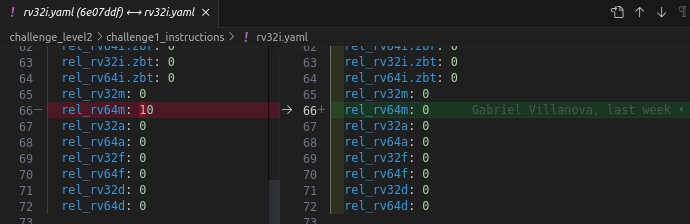
\includegraphics[width=0.48\textwidth]{./rv32i_diff.png}
    \caption{Updated code for AAPG generation in C2L1 bug.}
    \label{fig:rv32i_diff}
\end{figure}


By making this modification, the \texttt{aapg} will no longer generate RV64M instructions, ensuring that the assembler doesn't encounter any ``unrecognized opcode" errors as is shown in Figure \label{ref:unrec}.

\begin{figure}[H]
    \centering
    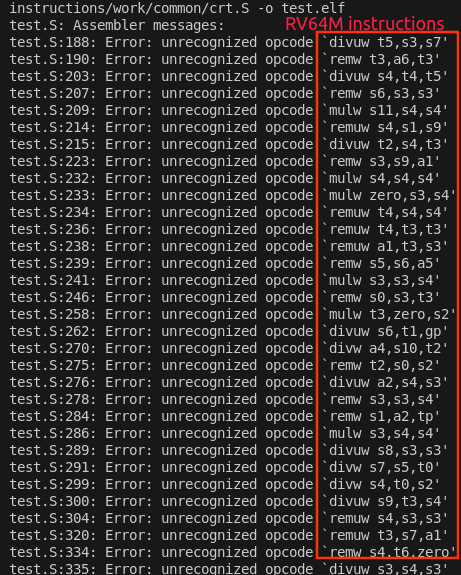
\includegraphics[width=0.48\textwidth]{./unrec_op.png}
    \caption{Unrecognized instruction error due to RV64M generation in AAPG.}
    \label{fig:unrec}
\end{figure}

% -------------------------------------------------------
% Challenge: AAPG Generation Test
% -------------------------------------------------------
\section{Challenge 2 Level 2 (C2L2): AAPG Generation Test}

In this Section, Challenge 2 Level 2 (C2L2) is presented. First, a description of the challenge is explained, second, the implementation to solve is presented, and finally, a discussion about the AAP tool is given. 

\subsection{Description}

The challenge is to create an AAPG (Automated Assembly Program Generator) config file that generates a test with 10 illegal exceptions, each with the correct handler code. This challenge aims to assess the ability to configure the AAPG tool to produce specific test cases with the desired number of illegal exceptions and their corresponding handlers.

\subsection{Solution}

To complete this challenge, the following steps were followed:

\begin{enumerate}
    \item The config file used in ``challenge\_level2/challenge\_instructions" was copied to this directory. The existing config file likely specified configurations for the RV32I base integer instruction set and other relevant parameters.
    \item The line in ``rv32i.yaml" was updated from:
    
\begin{minted}[frame=single]{nasm}
ecause02: 0
\end{minted}

    to:
    
\begin{minted}[frame=single]{nasm}
ecause02: 9
\end{minted}
    
    This modification sets the value of \texttt{ecause02} to 9, effectively instructing the AAPG to generate 10 illegal exceptions during the test.
    
    \item The AAPG tool was run to generate the assembly code based on the updated config file. The generated assembly code will contain the specified test cases with the desired illegal exceptions.
\end{enumerate}

The reason for using ``9" instead of "10" was due to the output log test, as shown in Figure \ref{fig:output_simulation}. Using ``9" resulted in 10 exceptions, in accordance with the challenge specification. 

\begin{figure}[h]
  \centering
  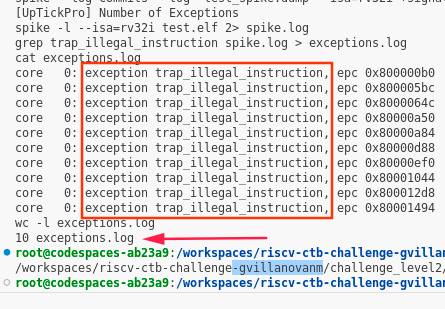
\includegraphics[width=0.47\textwidth]{./c2l2_img/img1.png}
  \caption{Output of the C2L2 simulation.}
  \label{fig:output_simulation}
\end{figure}

\subsection{How Is Exception Generated in AAPG?}

Configuring the \texttt{ecause02} fields and running AAPG will generate random assembly routines with exceptions. These routines are then incorporated into the \texttt{test.S} code, as shown in the figure below.

\begin{figure}[h]
  \centering
  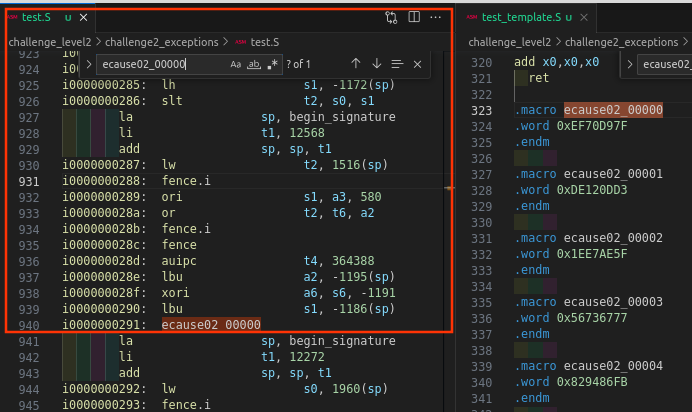
\includegraphics[width=1\linewidth]{./c2l2_img/expl.png}
  \caption{Code Generation Process}
\end{figure}

Each snippet will consist of a \texttt{.word} instruction, encompassing anything that does not meet the criteria for a legal instruction in the context of the system. This will cause an exception to be invoked.

This process resembles the challenge exercise found in \texttt{challenge\_level1/challenge3\_illegal}, where scenarios involving illegal instructions were encountered.

\subsection{AAPG Future Work}

When executing the config file presented in the last section, the output was not always the same. Sometimes, after execution, the simulation never stopped, and other times, the simulation stopped and returned the log presented in the last section.

Attempts were made to create some modifications in ``rv32i.yaml," but the same behavior persisted. It is suspected that there may be a bug in AAPG that causes this inconsistent behavior. Further investigation is needed to resolve this issue.

The inconsistent behavior observed during the AAPG execution raises concerns about the tool's reliability. It is crucial to investigate and address this issue to ensure consistent and accurate generation of assembly programs for testing and verification purposes.

\section{Challenge 3 Level 1 (C3L1): Capture The Bug - Given Design (\texttt{riscv\_buggy})}

This challenge involves using the AAPG to create an infrastructure that exposes bugs in the given design. In this section, the methodology or strategy used will be presented, along with its implementation, the results obtained, and finally the conclusion.

\subsection{C3L1: Methodology}

For verifying the Design Under Test (DUT), we have chosen the Functional Verification (FV) methodology. This choice is justified by the existing infrastructure, including the AAPG generation and the comparison method based on the "diff" command between the DUT and the Reference/Golden Model (refmod or spike). Other strategies, such as UVM or Formal Verification, could also be used, but they would require more software and RTL (Register Transfer Level) access.

The fundamental steps of the Functional Verification flow are as follows:

\begin{enumerate}
    \item Study Design;
    \item Define a Verification Plan (VP); 
    \item Implement the test;
    \item Measure, refine and validate (Results);
\end{enumerate}

The process must be repeated if the VP's goals was not reached, otherwise the verification is done. This process is applied to the given design and described in detail in the next Subsections.

\subsection{C3L1: STEP1 - Study Design}

The riscv\_buggy is a black-box RISC-V processor that supports RV32I (RISC-V 32-bit base integer instructions) and CSR (Control and Status Register) instructions (information gotten from Slack). 

Considering this level of knowledge about the system it's appropriate to implement a verification environment to test every instruction specified (RV32I and CSR instructions). The instruction set details are presented in the Annex section \cite{riscv_isa_vol1}. In a real scenario much more should be considered.

The next step is to define a Verification Plan.

\subsection{C3L1: STEP2 - Verification Plan (VP)}

In general, the Verification Plan (VP) is a document that defines the coverage specification, the tests that need to be implemented, and the test architecture.

Based on the information about the DUT, Reference Model (spike), and the AAPG tool, which assists in test creation, the coverage can be based on the expected instructions, and the tests can be designed to leverage the AAPG possibilities. In addition, the traditional verification architecture can be adapted with the available tools. These topics are presented further in the following subsections.

\subsubsection{Coverage Specification}

The verification environment must measure the stimulated instructions and check if all instructions - RV32I and CSR - were covered. It's a stop criterion.

\subsubsection{Test Specification}

In this context, the test specification was divided into 1) sequence generation and 2) test infrastructure (stimulus, comparison, and traceability). 

\paragraph{Sequences generation}

The sequences should be created using AAPG tool. The AAPG allows configuring the group of instructions which is better to understand the bugs. It can be done by configuring the fields in the YAML file. These fields are presented in Listing \ref{lst:c1l3_yaml}. 

\begin{listing}[h!]
\caption{AAPG Configuration.}
\label{lst:c1l3_yaml}
\begin{minted}[frame=single]{nasm}
total_instruction: <config>
rel_sys.csr: <config>
rel_rv32i.ctrl: <config>
rel_rv32i.compute: <config>
rel_rv32i.data: <config>
rel_rv32i.fence: <config>
\end{minted}
\end{listing}

The RV32I instructions can be considered as compute, data, fence, and ctrl. The csr is the Control and Status Register. The field <config> is a value or a weight that the AAPG uses to create the sequences randomly.

An important note is that the ``total\_of\_instructions" field in the first regressions should be kept equal to one or two. This is made to avoid false positives. For example, if a buggy instruction was executed, and its result was saved in register x7, any operation involving x7 could potentially be a false bug. Therefore, by keeping the ``total\_of\_instructions" small and increasing the number of tests, we improve the chances of capturing a real bug. Additionally, each test uses a new seed, which further increases the likelihood of finding a real bug. The planned tests are presented in the next paragraphs.

\paragraph{Test Architecture}

The test architecture is based on the traditional verification architecture, as shown in Figure \ref{fig:arch}. It includes the following steps:

\begin{enumerate}
    \item Stimulus generation represented as ``.bin"
    \item Driving the DUT and the Golden Model.
    \item Comparing the outputs.
    \item Extracting the results (scoreboard).
\end{enumerate}

\begin{figure}[H]
    \centering
    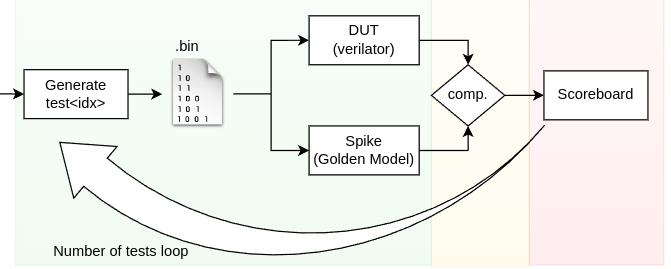
\includegraphics[width=0.5\textwidth]{./c3l1_img/arch.png}
    \caption{Traditional verification architecture adapted to the RISC-V verification environment.}
    \label{fig:arch}
\end{figure}

\subsection{C3L1: STEP1 - Test Implementation}

The sequences planned, and the details about the verification environment implementation are presented in this Section.

\subsubsection{Sequences}

The sequences were planned to separate the group of analysis due to the facilitate associate in analysis and debugging.

\paragraph{TEST\_ONLY\_DATA}

The configuration file is presented in Listing \ref{lst:c1l3_tod}. It will generate only data instructions (lw, sw, li, sh, lh, etc).

\begin{listing}[h!]
\caption{TEST\_ONLY\_DATA.}
\label{lst:c1l3_tod}
\begin{minted}[frame=single]{nasm}
  rel_sys.csr: 0
  rel_rv32i.ctrl: 0
  rel_rv32i.compute: 0
  rel_rv32i.data: 1
  rel_rv32i.fence: 0
\end{minted}
\end{listing}

\paragraph{TEST\_ONLY\_COMPUTE}

The configuration file is presented in Listing \ref{lst:c1l3_toc}. It will generate only compute instructions (or, xor, add, addi, sub, etc).

\begin{listing}[h]
\caption{TEST\_ONLY\_COMPUTE.}
\label{lst:c1l3_toc}
\begin{minted}[frame=single]{nasm}
  rel_sys.csr: 0
  rel_rv32i.ctrl: 0
  rel_rv32i.compute: 1
  rel_rv32i.data: 0
  rel_rv32i.fence: 0
\end{minted}
\end{listing}

\paragraph{TEST\_CSR\_DATA\_FENCE}

The configuration file is presented in Listing \ref{lst:c1l3_tcdf}. It will generate data, fence, and csr instructions. In this case, it's not possible to isolate CSR, then data and fence were set to allow the generation.s

In addition, the total instruction needs to be increased to fit the distribution specification.

\begin{listing}[ht]
\caption{TEST\_CSR\_DATA\_FENCE.}
\label{lst:c1l3_tcdf}
\begin{minted}[frame=single]{nasm}
    total_instructions: 3 # needed
    rel_sys.csr: 1 # focus
    rel_rv32i.ctrl: 0
    rel_rv32i.compute: 0 
    rel_rv32i.data: .5
    rel_rv32i.fence: .5
\end{minted}
\end{listing}

\paragraph{TEST\_CTRL\_DATA}

The configuration file is presented in Listing \ref{lst:c1l3}. It will generate Ctrl (control) and data instructions. Also, it's not possible to isolate Ctrl, then data was included in the generation.

In addition, the total instruction needs to be increased to fit the distribution specification.

\begin{listing}[h!]
\caption{TEST\_CTRL\_DATA.}
\label{lst:c1l3}
\begin{minted}[frame=single]{nasm}
    total_instructions: 500
    rel_sys.csr: 0 
    rel_rv32i.ctrl: 0.2 # focus
    rel_rv32i.compute: 0 
    rel_rv32i.data: 2
    rel_rv32i.fence: 0
    \end{minted}
\end{listing}

\subsubsection{Test Implementation}

The test infrastructure was implemented in Python (file: \texttt{run\_tests.py}) in three steps, as shown in Figure \ref{fig:implement}.

\begin{figure*} % Use figure* to make the figure span the whole page
    \centering
    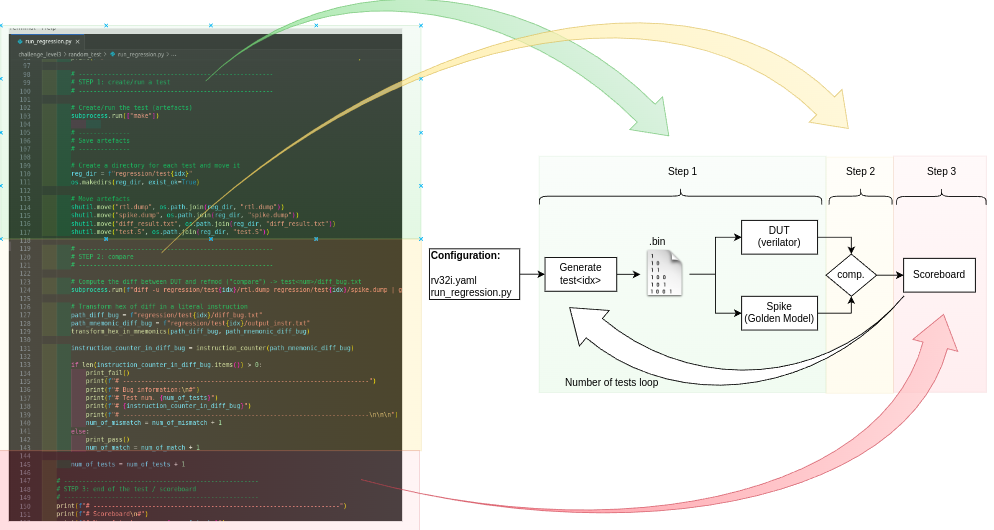
\includegraphics[width=1\textwidth]{./c3l1_img/implement.png} % This sets the image width to the text width
    \caption{Steps for the test implementation.}
    \label{fig:implement}
\end{figure*}

The routines are based on these three steps. Step 1 calls the Makefile (\# make) and performs the following actions: AAPG generation, cross-compilation of the generated test.S using the RISC-V Toolchain, stimulation (spike and verilator dut), and comparison of the models' outputs using the ``diff" command. Step 2 reads the generated ``diff" file, verifies if it is empty or not, and increments the ``match" variable with a PASS message if it is empty, or increments the ``mismatch" variable and presents information about the bug (see Figure \ref{fig:fail}). Finally, Step 3 prints the scoreboard as shown in Figure \ref{fig:scb}. 

Before executing this script, the test configuration (TEST\_ONLY\_DATA, TEST\_ONLY\_COMPUTE, etc.) and the number of tests (set by the variable ``num\_of\_tests" inside \texttt{run\_tests.py}) must be defined. After that, the script can be run (\# python3 \texttt{run\_tests.py}). The main infrastructure is based on the last challenges learned.

\begin{figure}[H]
    \centering
    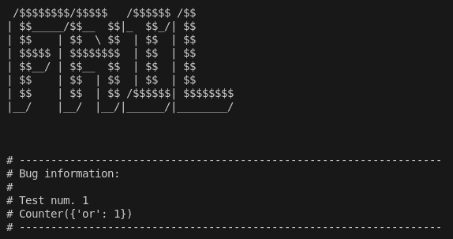
\includegraphics[width=0.47\textwidth]{./c3l1_img/fail.png}
    \caption{Bug information presentation.}
    \label{fig:fail}
\end{figure}

\begin{figure}[H]
    \centering
    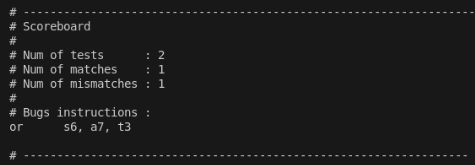
\includegraphics[width=0.48\textwidth]{./c3l1_img/scb.png}
    \caption{Scoreboard presentation.}
    \label{fig:scb}
\end{figure}

Another script (\texttt{run\_analysis\_reg.py}) was implemented for generating histograms and conducting coverage analysis. After executing regressions (see Figure \ref{fig:regressions_sample}), this script reads the generated artifacts, calculates the number of executed instructions and their percentage, plots the histogram, and calculates the percentage of instructions exercised compared to all expected instructions (Annex). In summary, it implements the coverage analysis by reading the dump files, applying disassembly, and measuring the instructions from that.

\begin{figure}[H]
    \centering
    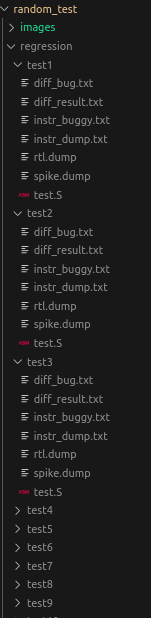
\includegraphics[width=0.19\textwidth]{./c3l1_img/regressions_sample.png}
    \caption{Sample of regressions execution.}
    \label{fig:regressions_sample}
\end{figure}

The results obtained from applying the defined Methodology will be presented in this section, along with the bugs found. 

\subsection{C3L1 Results: TEST\_ONLY\_DATA - Regression 1}

\subsubsection{Configuration}

\begin{itemize}
    \item num\_of\_tests = 10
    \item total\_instructions = 2
\end{itemize}

\subsubsection{Result}
PASS.

\begin{figure}[H]
    \centering
    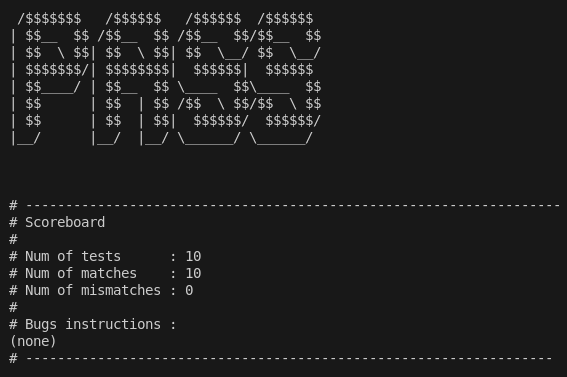
\includegraphics[width=0.47\textwidth]{./c3l1_img/tod_10_r.png}
    \caption{Regression 1 results for TEST\_ONLY\_DATA.}
    \label{fig:tod\_10\_r}
\end{figure}

\subsubsection{Histogram of instructions stimulated}

Even configuring only data, the initialization of the system uses other instructions, then this is captured in the analysis.

\subsection{C3L1 Results: TEST\_ONLY\_DATA - Regression 2}


\subsubsection{Configuration}
\begin{itemize}
    \item num\_of\_tests = 100
    \item total\_instructions = 20
\end{itemize}

\subsubsection{Result}
PASS.

\begin{figure}[H]
    \centering
    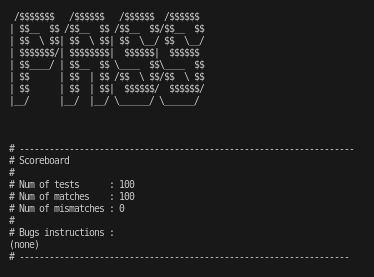
\includegraphics[width=0.53\textwidth]{./c3l1_img/tod_100_r.png}
    \caption{Regression 2 results for TEST\_ONLY\_DATA.}
    \label{fig:tod_100_r}
\end{figure}

\subsubsection{Histogram of instructions stimulated}

The instructions kept the same but the frequency increased compared to regression 1 (see Figure \ref{fig:tod_10}
 and \ref{fig:tod_100}.
 
\begin{figure}[ht]
    \centering
    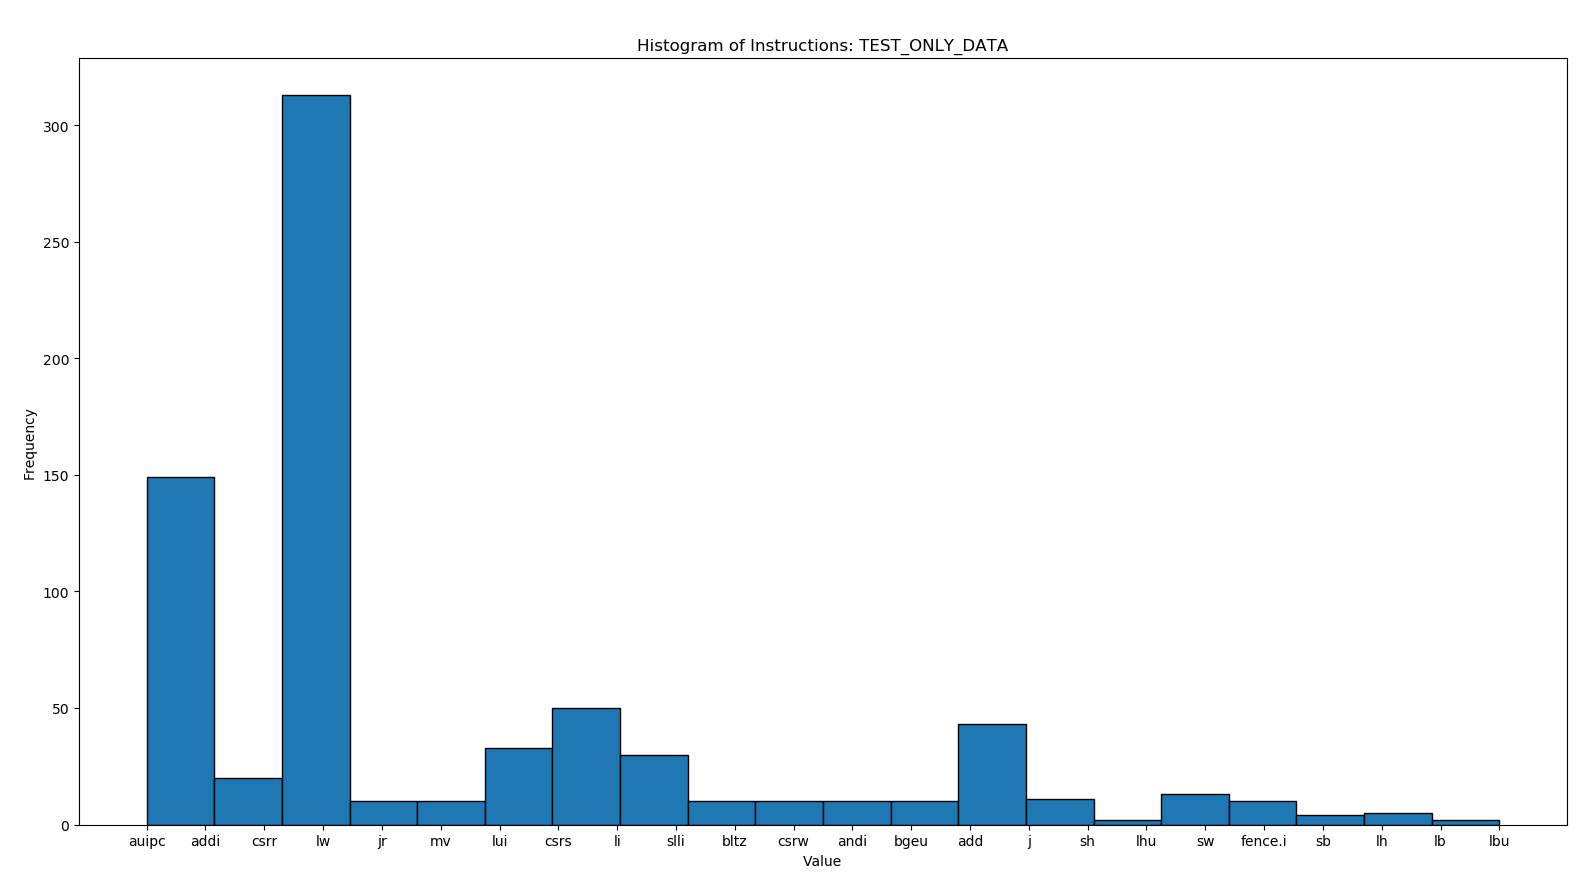
\includegraphics[width=0.48\textwidth]{./c3l1_img/tod_10.png}
    \caption{Histogram of instructions stimulated for TEST\_ONLY\_DATA (regression 1).}
    \label{fig:tod_10}
\end{figure}


\subsubsection{Discussion and Coverage Status}

Two regressions were executed. The first one with 10 tests and 2 instructions, but no bugs were encountered. The second regression, with 100 tests and 20 instructions, still did not find any bugs. It suggests that the bug might not be in the RV32I.data set (see the histogram).

The coverage was calculated for this case and, as expected, it did not reach 100\% since it is a subset of all instructions.

\begin{figure}[H]
    \centering
    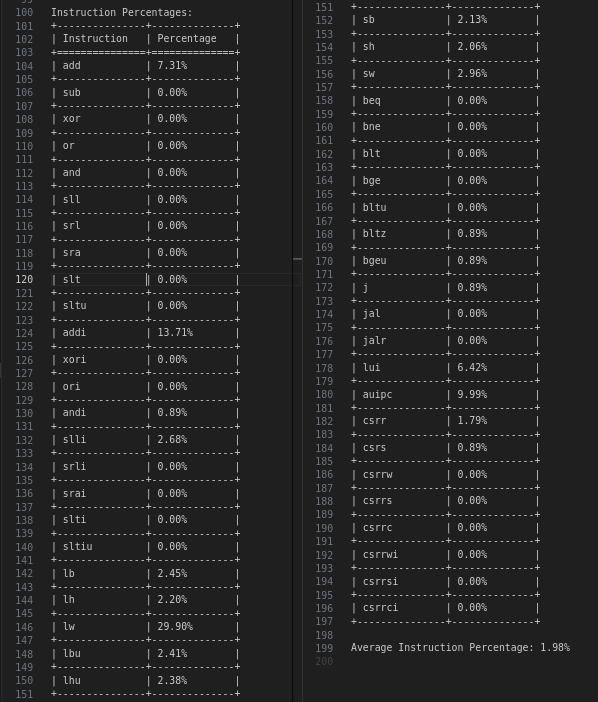
\includegraphics[width=0.48\textwidth]{./c3l1_img/cov_t0.png}
    \caption{Coverage for TEST\_ONLY\_DATA.}
    \label{fig:cov_t0}
\end{figure}

\begin{verbatim}
Instructions Tested: 24/47
Percentage Instructions Tested: 51.06%
\end{verbatim}

\begin{figure}[H]
    \centering
    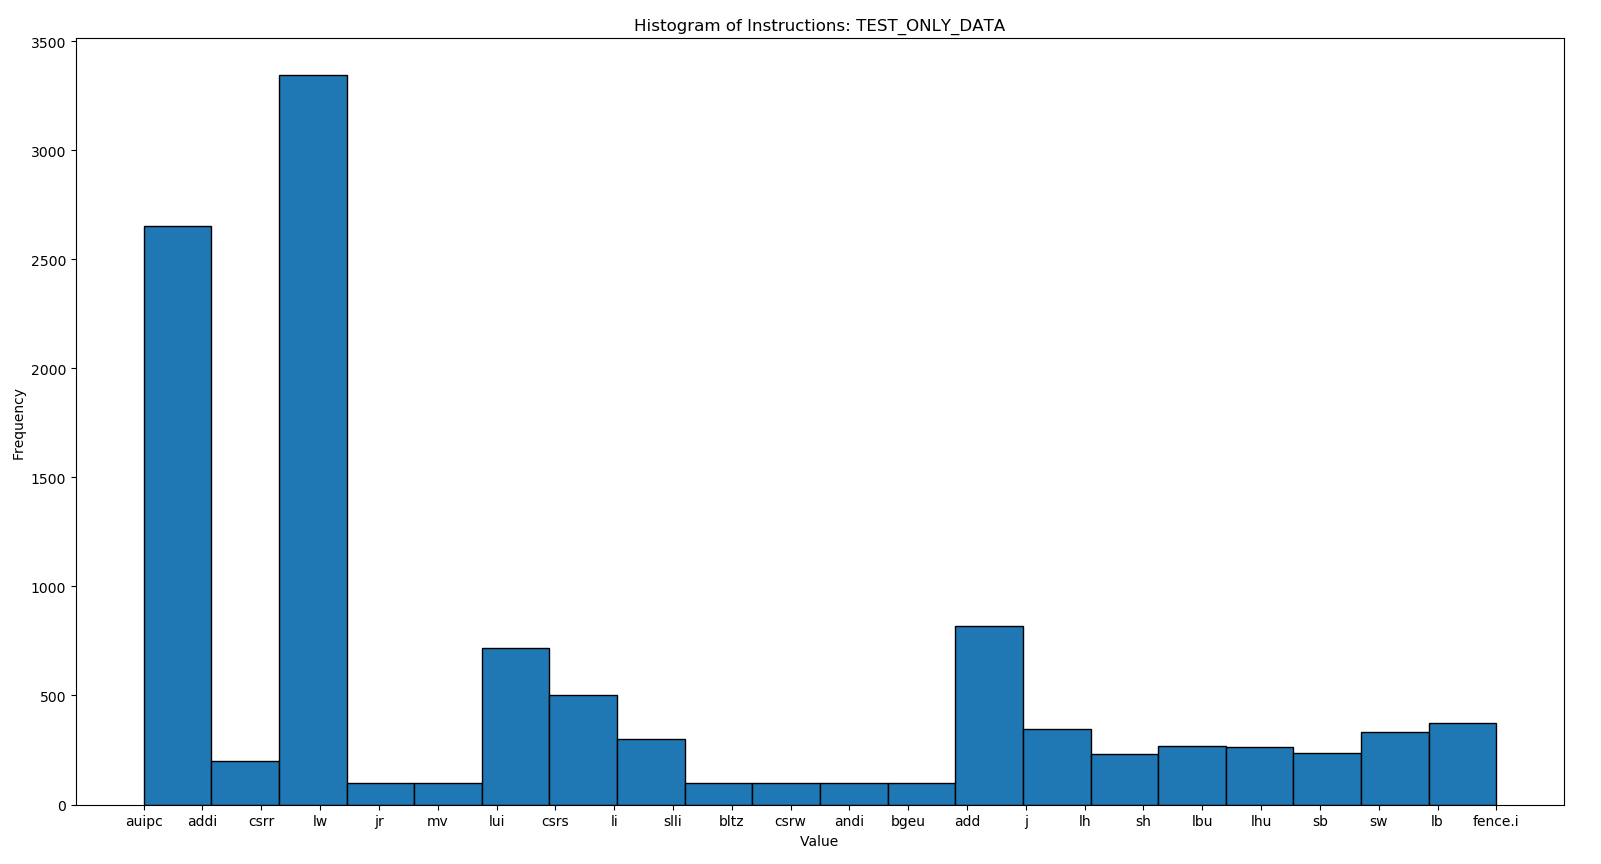
\includegraphics[width=0.5\textwidth]{./c3l1_img/tod_100.png}
    \caption{Histogram of instructions stimulated for TEST\_ONLY\_DATA (regression 2).}
    \label{fig:tod_100}
\end{figure}

\subsection{C3L1 Results: TEST\_ONLY\_COMPUTE-Regression1}

\subsubsection{Configuration}

\begin{itemize}
    \item num\_of\_tests = 10
    \item total\_instructions = 2
\end{itemize}

\subsubsection{Result}
The scoreboard captured bugs in the instructions compute OR and ORI. An deep investigation is presented after regressions.

\begin{figure}[H]
    \centering
    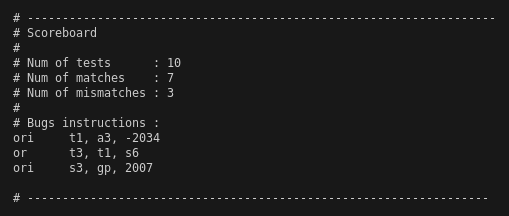
\includegraphics[width=0.5\textwidth]{./c3l1_img/toc_10_r.png}
    \caption{Regression 1 results for TEST\_ONLY\_COMPUTE.}
    \label{fig:toc_10_r}
\end{figure}

\subsubsection{Histogram of instructions stimulated}
as expected the compute instructions are presented.

\begin{figure}[H]
    \centering
    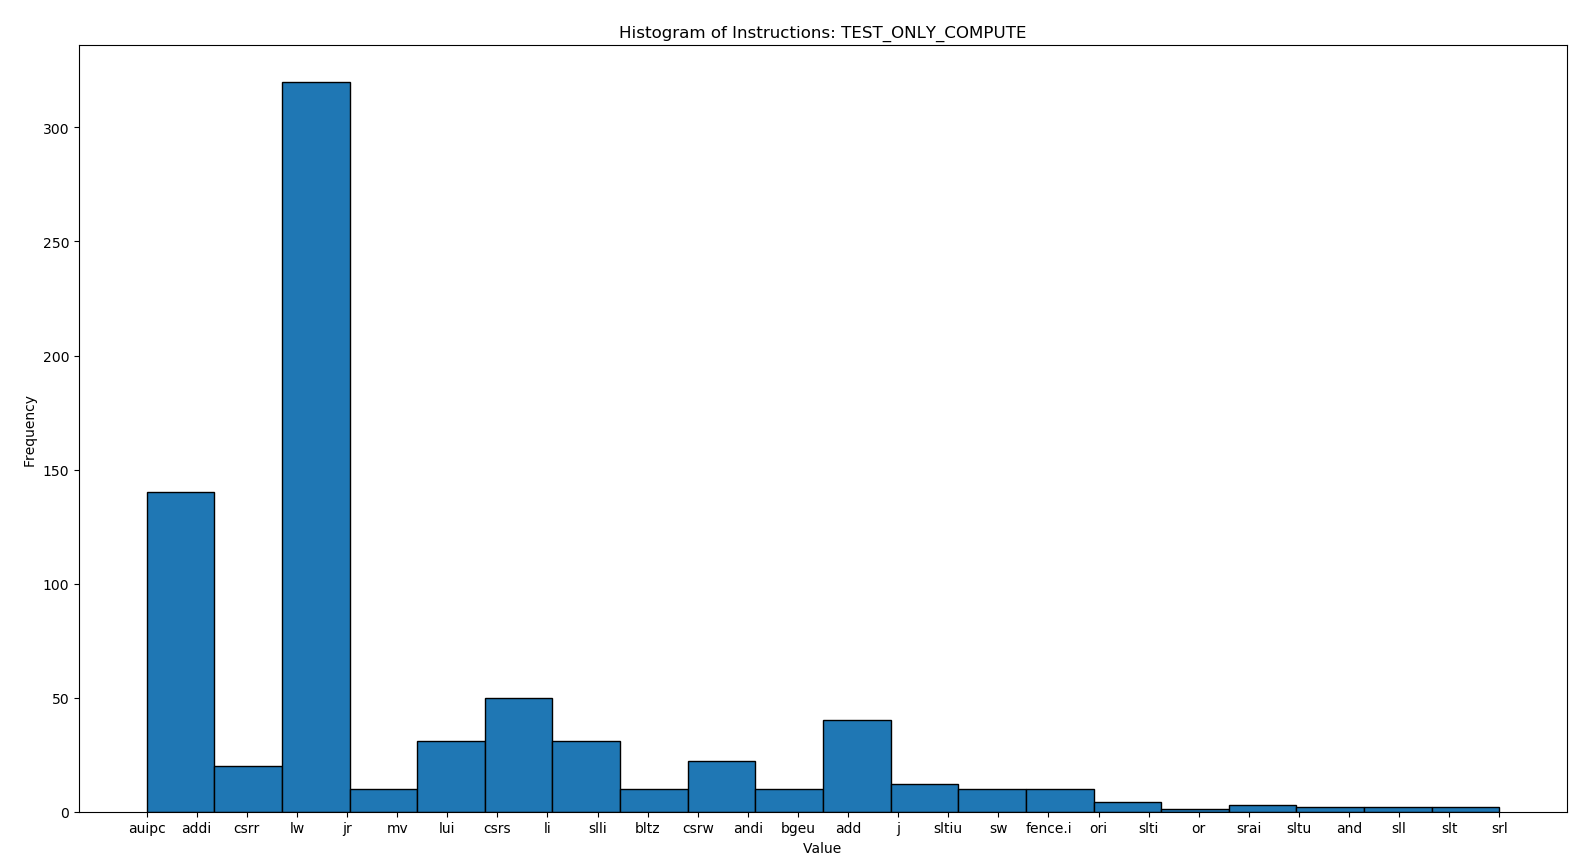
\includegraphics[width=0.48\textwidth]{./c3l1_img/toc_10.png}
    \caption{Histogram of instructions stimulated for TEST\_ONLY\_COMPUTE.}
    \label{fig:toc_10}
\end{figure}

\subsection{C3L1 Results: TEST\_ONLY\_COMPUTE-Regression2}

\subsubsection{Configuration}

\begin{itemize}
    \item num\_of\_tests = 100
    \item total\_instructions = 2
\end{itemize}

\subsubsection{Result}
Scoreboard.

\begin{figure}[H]
    \centering
    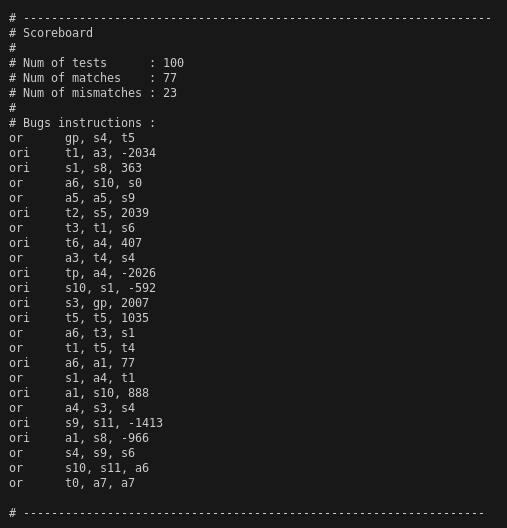
\includegraphics[width=0.47\textwidth]{./c3l1_img/toc_100_r.png}
    \caption{Regression 2 results for TEST\_ONLY\_COMPUTE.}
    \label{fig:toc_100_r}
\end{figure}

\subsubsection{Histogram of instructions stimulated}
as expected the compute instructions are presented.


\begin{figure}[H]
    \centering
    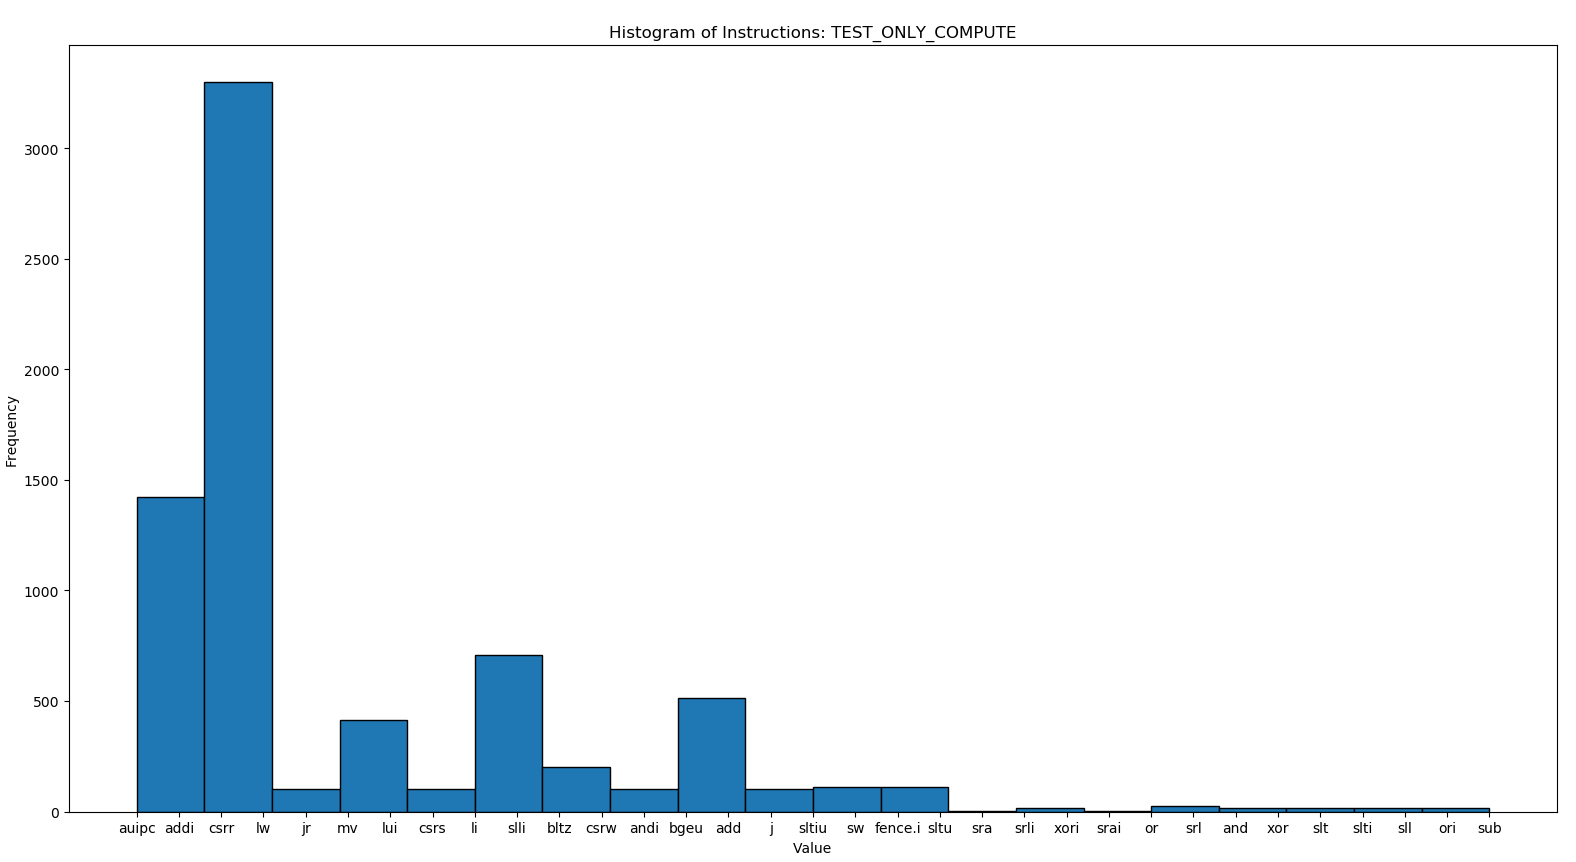
\includegraphics[width=0.5\textwidth]{./c3l1_img/toc_100.png}
    \caption{Histogram of instructions stimulated for TEST\_ONLY\_COMPUTE.}
    \label{fig:toc_100}
\end{figure}

\subsubsection{Discussion and Coverage Status}

The test captured a bug in the OR and ORI instruction. To understand the cause of the bug, let's consider the scenario presented below.

\begin{figure*}
    \centering
    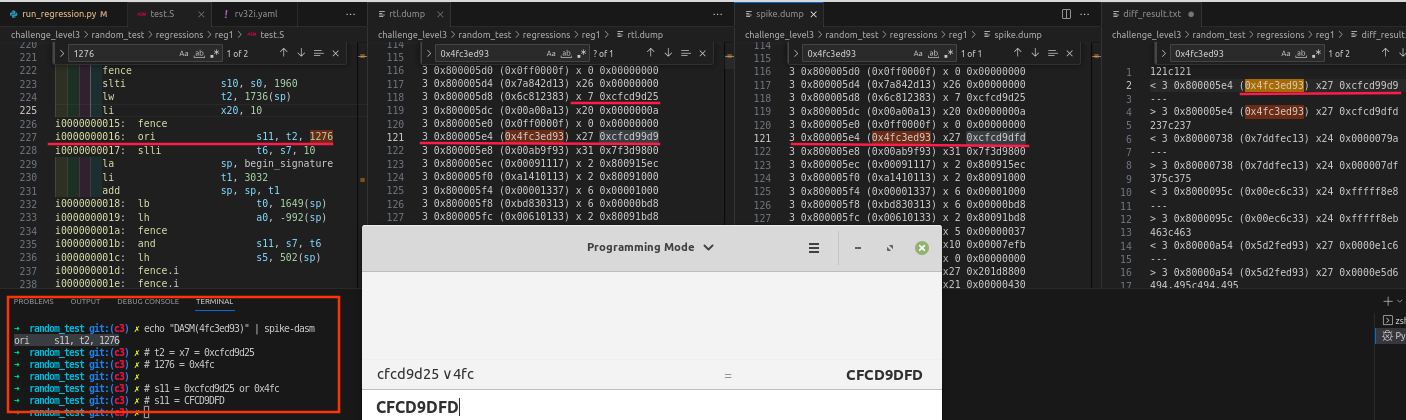
\includegraphics[width=1\textwidth]{./c3l1_img/ori_bug_anal2.png}
    \caption{Analysis of the ORI bug.}
    \label{fig:ori_bug_anal2}
\end{figure*}

By analyzing the literal operation (Figure \ref{fig:ori_bug_anal}), it's possible to understand the real cause of the bug. When A and B are equal to 1, the output bit expected is inverted. The OR instruction also has a similar bug, and the same analysis can be done to verify the cause in detail.

\begin{figure}[H]
    \centering
    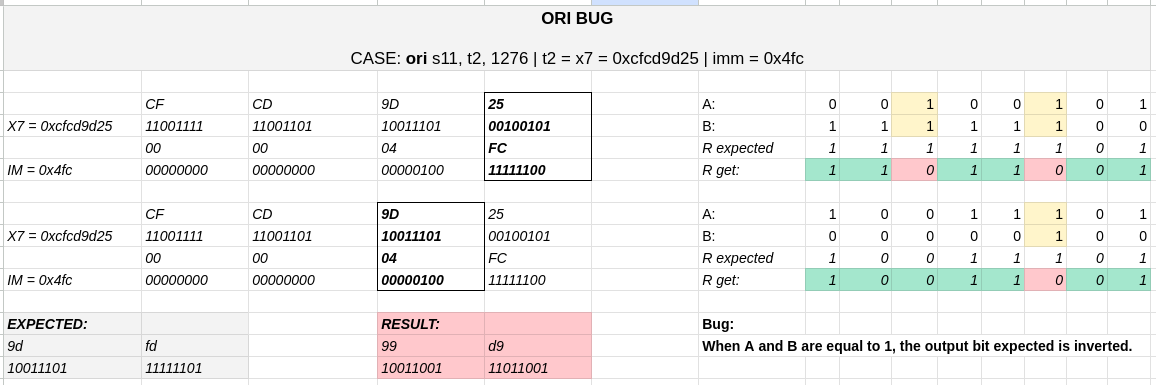
\includegraphics[width=0.5\textwidth]{./c3l1_img/ori_bug_anal.png}
    \caption{Analysis of the ORI bug.}
    \label{fig:ori_bug_anal}
\end{figure}

\textbf{Important note: }Increasing the number of instructions in this test will return many bugs. However, without accurate analysis, it's hard to identify if it is a real bug or generated due to the wrong value assigned to registers after the OR or ORI operation creating a false positive (or "fake" bug). Therefore, it's safer and easier, in terms of bug capture, to keep the number of instructions equal to one or two and increase the number of tests.

\subsubsection{Coverage}

The coverage was calculated in regression 2, and the result is shown below. The increase in coverage is due to the set of instructions configured. The compute set (add, xor, xori, etc.) is greater than the compute data set. As a result, the coverage reached 70.21\%.

\begin{verbatim}
Instructions Tested: 33/47
Percentage Instructions Tested: 70.21%
\end{verbatim}

\subsection{C3L1 Results: TEST\_CSR\_DATA\_FENCE - Regr. 1}

\subsubsection{Configuration}

\begin{itemize}
    \item num\_of\_tests = 30
    \item total\_instructions = 3
\end{itemize}

\subsubsection{Result}

No bugs were encountered in this case.

\subsection{C3L1 Results: TEST\_CSR\_DATA\_FENCE - Regr. 2}

\subsubsection{Configuration}

\begin{itemize}
    \item num\_of\_tests = 30
    \item total\_instructions = 10
\end{itemize}

\subsubsection{Result}
The instruction \textbf{csrrci} appears in the Spike dump but not in the RTL dump due to this inconsistency the test environment returns a bug as presented in Figure \ref{fig:tcdf_reg2}). However, apparently the bug is related to the tool and not to the design. As a result, it will be not considered a bug in riscv\_buggy.

\begin{figure}[H]
    \centering
    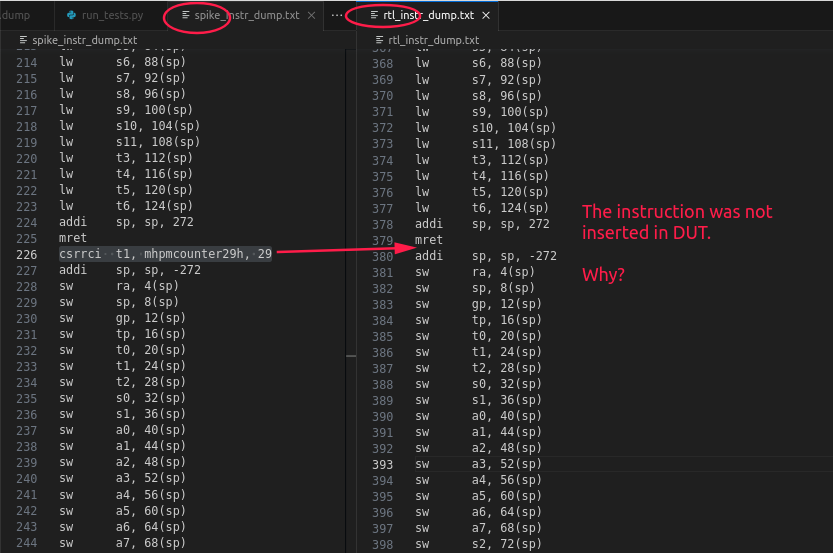
\includegraphics[width=0.5\textwidth]{./c3l1_img/tcdf_reg2.png}
    \caption{Regression 2 results for TEST\_CSR\_DATA\_FENCE.}
    \label{fig:tcdf_reg2}
\end{figure}

\subsection{C3L1 Results: TEST\_CTRL\_DATA}

The method was executed under this configuration, and it demonstrated exceptional stability with no encountered bugs, even during exhaustive stimulation.

\subsection{C3L1: Conclusion riscv\_buggy}

Based on the tested extensions and strategy, the result of riscv\_buggy verification is summarized below. In other words, the tests encountered bugs in the OR and ORI instructions and a inconsistency in CSR.

\begin{verbatim}
# Extension        # RESULT/STATUS
rel_sys.csr        # INCONSISTENT
rel_rv32i.ctrl:    # NO BUGS
rel_rv32i.compute: # BUGS: OR/ORI instr.
rel_rv32i.data:    # NO BUGS
rel_rv32i.fence:   # NO BUGS
\end{verbatim}

Considering all the regression results, the specified coverage reaches 100\%. However, it is important to note that due to the encountered bugs, merging the results might not provide a meaningful representation of the overall coverage in this case. The identified bugs should be carefully addressed and resolved before concluding the final coverage assessment.

In a real development flow, these results should be discussed with the designer responsible to address the problems. After that, the same tests should pass, and finally, a refinement in the VP also should be made to stimulate in different ways the design and achieve coverage. % riscv_buggy
\section{Challenge 3 Level 2 (C3L2): RISCV-DV Test Coverage Enhancement}

\subsection{Introduction}
The objective of this activity was to improve test coverage in the RISCV-DV tool for the rv32i ISA. Despite various configurations being tested and evaluated, achieving 100\% coverage was challenging due to time constraints, lack of documentation, and limited knowledge of the tool.

\subsection{Test Generation and Interaction}
RISCV-DV was used for test generation with the following command:

\begin{verbatim}
run --target rv32i --test riscv_arithm
etic_basic_test --testlist testlist.yaml
--simulator pyflow
\end{verbatim}

To control the number of tests, the \texttt{-i} (interaction) parameter was utilized. For instance:

\begin{verbatim}
run --target rv32i --test riscv_arithm
etic_basic_test --testlist testlist.yaml
--simulator pyflow -v -i 50
\end{verbatim}

This command generated 50 tests as observed in Figure \ref{fig:run1}.

\begin{figure}[h]
  \centering
  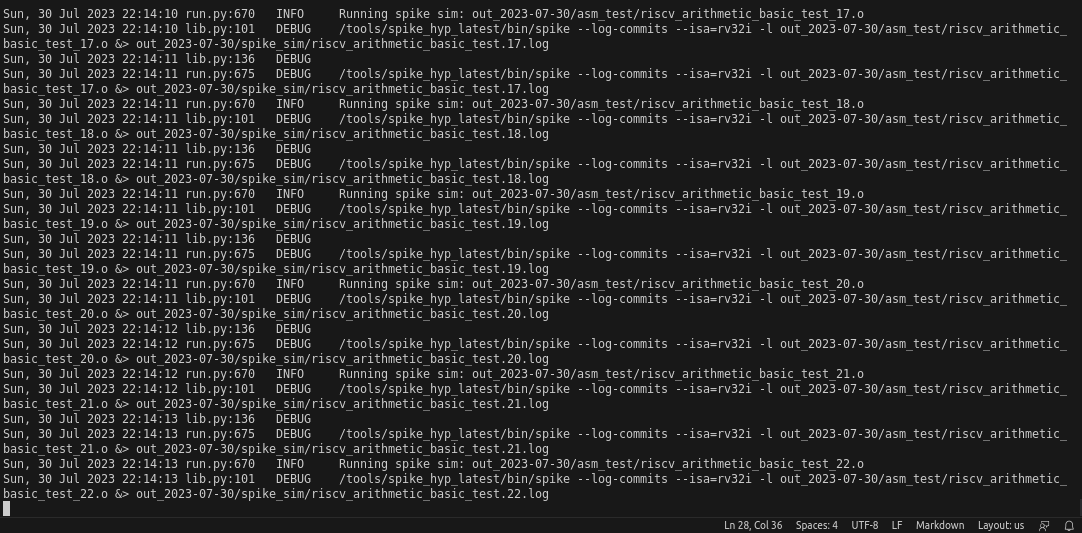
\includegraphics[width=0.5\textwidth]{./c3l2_img/run1.png}
  \caption{Test Generation with Interaction}
  \label{fig:run1}
\end{figure}

\subsection{Test Analysis and Coverage}
The generated tests can be analyzed as shown in Figure \ref{fig:run2}.

Coverage information can be obtained using the \texttt{cov} tool with the command below. The resulting output is depicted in Figure \ref{fig:run3}.

\begin{verbatim}
cov --dir out_*/spike_sim --enable_visua
lization  --simulator pyflow
\end{verbatim}

To analyze the coverage metrics, it is necessary to read the \texttt{CoverageReport.txt} in the \texttt{cov\_*/} folder, as demonstrated in Figure \ref{fig:run4}.

\subsection{Conclusion and Next Steps}
While various configurations were tested and evaluated, achieving 100\% coverage was not realized due to the limited availability of documentation, time constraints, and unfamiliarity with the tool.

For future improvements, it is essential to explore the tool's documentation and seek assistance from the community to address the coverage issues efficiently. Additionally, further analysis of uncovered areas in the ISA and targeted test generation could be performed to enhance coverage results.

\begin{figure}[h]
  \centering
  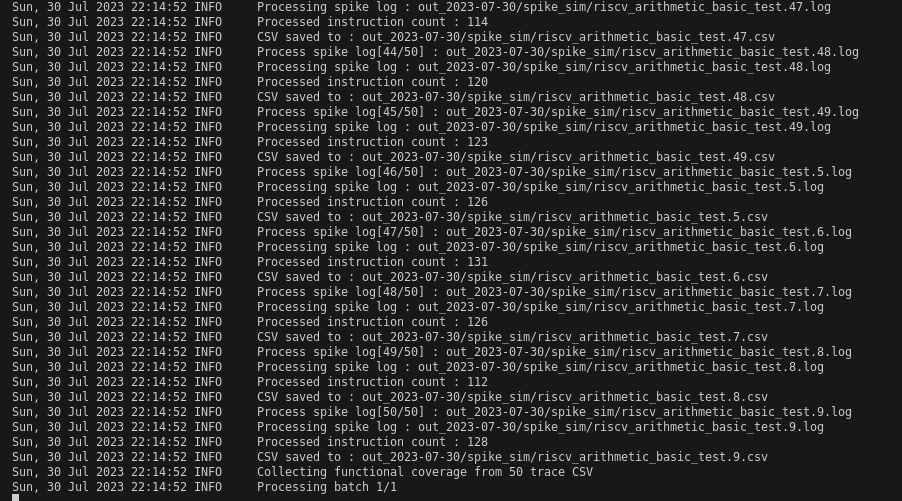
\includegraphics[width=0.5\textwidth]{./c3l2_img/run3.png}
  \caption{Coverage Report}
  \label{fig:run3}
\end{figure}

\begin{figure}[h]
  \centering
  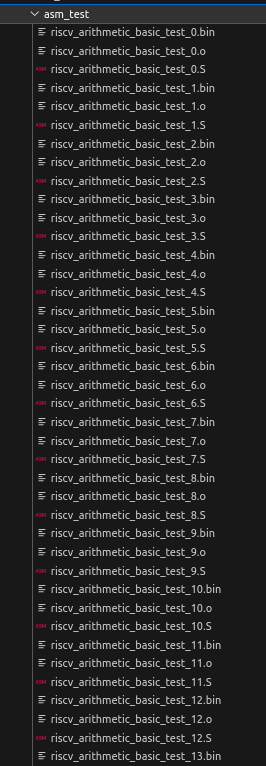
\includegraphics[width=0.21\textwidth]{./c3l2_img/run2.png}
  \caption{Test Analysis}
  \label{fig:run2}
\end{figure}


\begin{figure}[h]
  \centering
  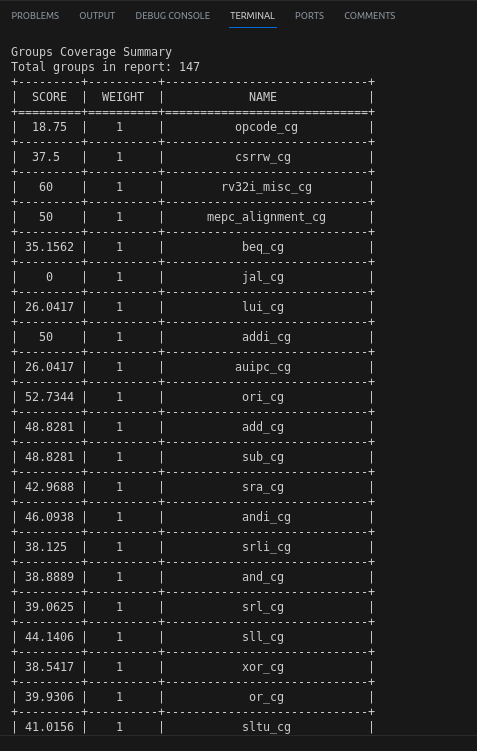
\includegraphics[width=0.19\textwidth]{./c3l2_img/run4.png}
  \caption{Coverage Metrics}
  \label{fig:run4}
\end{figure}

 % riscv_dv

% Annex
% DO NOT REMOVE THIS COMMAND
\addtolength{\textheight}{-12cm}

\begin{thebibliography}{99}

\bibitem{riscv_isa_vol1}
Andrew Waterman, Krste Asanovi\'c. (2019, December 13). \textit{The RISC-V Instruction Set Manual, Volume I: Unprivileged ISA}. SiFive Inc., CS Division, EECS Department, University of California, Berkeley. Retrieved from \url{https://inst.eecs.berkeley.edu/~cs61c/fa17/img/riscvcard.pdf}


\end{thebibliography}



\section{Annex}

\subsection{ISC-V RV32I Base Integer Instructions Card (to be reviewed)}

\begin{table*}[h] % Use table* instead of table to span both columns
    \centering
    \begin{tabular*}{\textwidth}{|c|c|c|c|c|c|l|} % Set the width of the tabular* environment to \textwidth
        \hline
        Instruction & Type   & Opcode   & funct3 & funct7 & Format & Description\\\hline
        ADD         & R-Type & 0110011  & 0x0    & 0x00   & rd = rs1 + rs2 & Add                              \\ \hline
        SUB         & R-Type & 0110011  & 0x0    & 0x20   & rd = rs1 - rs2 & Subtract                         \\ \hline
        XOR         & R-Type & 0110011  & 0x4    & 0x00   & rd = rs1 \^ rs2 & XOR (Bitwise Exclusive OR)       \\ \hline
        OR          & R-Type & 0110011  & 0x6    & 0x00   & rd = rs1 $||$ rs2 & OR (Bitwise OR)                  \\ \hline
        AND         & R-Type & 0110011  & 0x7    & 0x00   & rd = rs1 \& rs2 & AND (Bitwise AND)                \\ \hline
        SLL         & R-Type & 0110011  & 0x1    & 0x00   & rd = rs1 << rs2 & Shift Left Logical               \\ \hline
        SRL         & R-Type & 0110011  & 0x5    & 0x00   & rd = rs1 >> rs2 & Shift Right Logical              \\ \hline
        SRA         & R-Type & 0110011  & 0x5    & 0x20   & rd = rs1 >> rs2 (msb-extended) & Shift Right Arithmetic   \\ \hline
        SLT         & R-Type & 0110011  & 0x2    & 0x00   & rd = (rs1 < rs2) ? 1 : 0 & Set Less Than              \\ \hline
        SLTU        & R-Type & 0110011  & 0x3    & 0x00   & rd = (rs1 < rs2) ? 1 : 0 (zero-ext.) & Set Less Than (Unsigned) \\ \hline
        ADDI        & I-Type & 0010011  & 0x0    & -      & rd = rs1 + imm & Add Immediate                  \\ \hline
        XORI        & I-Type & 0010011  & 0x4    & -      & rd = rs1 \^ imm & XOR Immediate                  \\ \hline
        ORI         & I-Type & 0010011  & 0x6    & -      & rd = rs1 $||$ imm & OR Immediate                   \\ \hline
        ANDI        & I-Type & 0010011  & 0x7    & -      & rd = rs1 \& imm & AND Immediate                  \\ \hline
        SLLI        & I-Type & 0010011  & 0x1    & 0x00   & rd = rs1 << imm[0:4] & Shift Left Logical Immediate   \\ \hline
        SRLI        & I-Type & 0010011  & 0x5    & 0x00   & rd = rs1 >> imm[0:4] & Shift Right Logical Immediate  \\ \hline
        SRAI        & I-Type & 0010011  & 0x5    & 0x20   & rd = rs1 >> imm[0:4] (msb-extended) & Shift Right Arithmetic Immediate \\ \hline
        SLTI        & I-Type & 0010011  & 0x2    & -      & rd = (rs1 < imm) ? 1 : 0 & Set Less Than Immediate    \\ \hline
        SLTIU       & I-Type & 0010011  & 0x3    & -      & rd = (rs1 < imm) ? 1 : 0 (zero-ext.) & Set Less Than Immediate (Unsigned) \\ \hline
        LB          & I-Type & 0000011  & 0x0    & -      & rd = M[rs1 + imm][0:7] & Load Byte                  \\ \hline
        LH          & I-Type & 0000011  & 0x1    & -      & rd = M[rs1 + imm][0:15] & Load Half                  \\ \hline
        LW          & I-Type & 0000011  & 0x2    & -      & rd = M[rs1 + imm][0:31] & Load Word                  \\ \hline
        LBU         & I-Type & 0000011  & 0x4    & -      & rd = M[rs1 + imm][0:7] (zero-ext.) & Load Byte (Unsigned)     \\ \hline
        LHU         & I-Type & 0000011  & 0x5    & -      & rd = M[rs1 + imm][0:15] (zero-ext.) & Load Half (Unsigned)     \\ \hline
        SB          & S-Type & 0100011  & 0x0    & -      & M[rs1 + imm][0:7] = rs2[0:7] & Store Byte                     \\ \hline
        SH          & S-Type & 0100011  & 0x1    & -      & M[rs1 + imm][0:15] = rs2[0:15] & Store Half                   \\ \hline
        SW          & S-Type & 0100011  & 0x2    & -      & M[rs1 + imm][0:31] = rs2[0:31] & Store Word                   \\ \hline
        BEQ         & B-Type & 1100011  & 0x0    & -      & if (rs1 == rs2) PC += imm & Branch if Equal                \\ \hline
        BNE         & B-Type & 1100011  & 0x1    & -      & if (rs1 != rs2) PC += imm & Branch if Not Equal            \\ \hline
        BLT         & B-Type & 1100011  & 0x4    & -      & if (rs1 < rs2) PC += imm & Branch if Less Than            \\ \hline
        BGE         & B-Type & 1100011  & 0x5    & -      & if (rs1 >= rs2) PC += imm & Branch if Greater Than or Equal \\ \hline
        BLTU        & B-Type & 1100011  & 0x6    & -      & if (rs1 < rs2) PC += imm (unsigned) & Branch if Less Than \\ \hline
        BGEU        & B-Type & 1100011  & 0x7    & -      & if (rs1 >= rs2) PC += imm (unsigned) & Branch if Greater Than or Equal \\ \hline
        JAL         & J-Type & 1101111  & -      & -      & rd = PC + 4; PC += imm & Jump and Link               \\ \hline
        JALR        & I-Type & 1100111  & 0x0    & -      & rd = PC + 4; PC = rs1 + imm & Jump and Link Register . . . .  . . . . ....... \\ \hline
    \end{tabular*}
    \caption{RISC-V RV32I Base Integer Instructions Card.}
    \label{tab:rv32i_card}
\end{table*}



\end{document}
